\documentclass[12pt, oneside]{article}

\usepackage[letterpaper, scale=0.89, centering]{geometry}
\usepackage{fancyhdr}
\setlength{\parindent}{0em}
\setlength{\parskip}{1em}

\usepackage{tikz}
\usetikzlibrary{automata,positioning,arrows}

\pagestyle{fancy}
\fancyhf{}
\renewcommand{\headrulewidth}{0pt}
\rfoot{\href{https://creativecommons.org/licenses/by-nc-sa/2.0/}{CC BY-NC-SA 2.0} Version \today~(\thepage)}

\usepackage{amssymb,amsmath,pifont,amsfonts,comment,enumerate,enumitem}
\usepackage{currfile,xstring,hyperref,tabularx,graphicx,wasysym}
\usepackage[labelformat=empty]{caption}
\usepackage{xcolor}
\usepackage{multicol,multirow,array,listings,tabularx,lastpage,textcomp,booktabs}

\lstnewenvironment{algorithm}[1][] {   
    \lstset{ mathescape=true,
        frame=tB,
        numbers=left, 
        numberstyle=\tiny,
        basicstyle=\rmfamily\scriptsize, 
        keywordstyle=\color{black}\bfseries,
        keywords={,procedure, div, for, to, input, output, return, datatype, function, in, if, else, foreach, while, begin, end, }
        numbers=left,
        xleftmargin=.04\textwidth,
        #1
    }
}
{}

\newcommand\abs[1]{\lvert~#1~\rvert}
\newcommand{\st}{\mid}

\newcommand{\cmark}{\ding{51}}
\newcommand{\xmark}{\ding{55}}
 
\begin{document}
\begin{flushright}
    \StrBefore{\currfilename}{.}
\end{flushright} \section*{Day25}





Two models of computation are called {\bf equally expressive} when 
every language recognizable with the first model is recognizable with the second, and vice versa.

True / False: NFAs and PDAs are equally expressive.

True / False: Regular expressions and CFGs are equally expressive.


{\bf  Church-Turing Thesis} (Sipser p. 183): The informal notion of algorithm is formalized completely  and correctly by the 
formal definition of a  Turing machine. In other words: all reasonably expressive models of 
computation are equally expressive with the standard Turing machine.


\begin{center}
{\large \it  Some examples of models that are {\bf equally expressive} with deterministic Turing machines: }
\end{center}

\vfill

\fbox{ {\bf May-stay}  machines }
The May-stay machine model is the same as the usual Turing machine model,  except that
on each transition, the tape head may move L, move R, or Stay. 

Formally: $(Q, \Sigma, \Gamma, \delta, q_0, q_{accept}, q_{reject})$ where 
\[
  \delta: Q \times \Gamma \to Q \times \Gamma \times \{L, R, S\}
\]

{\bf Claim}: Turing machines and May-stay machines are equally expressive. {\it To prove \ldots}

To translate a standard TM to a may-stay machine: never use the direction $S$!


To translate one  of the  may-stay machines to standard TM:
any time TM would Stay, move right  then  left.

\begin{comment}
Formally: suppose $M_S =  (Q, \Sigma, \Gamma, \delta, q_0, q_{acc}, q_{rej})$
has $\delta: Q \times \Gamma \to Q \times \Gamma \times \{L, R, S\}$. Define
the Turing-machine
\[
  M_{new} =  (\phantom{\hspace{2.5in}})
\]

\vfill


\phantom{$M_{new}$ construction here \vspace{400pt}}
\vfill
\end{comment}

\vfill 

\fbox{ {\bf Multitape Turing machine}} A multitape Turing machine with $k$ tapes
can be formally represented as 
$(Q, \Sigma,  \Gamma, \delta, q_0, q_{acc}, q_{rej})$ 
where $Q$ is the finite set of  states,
$\Sigma$ is the  input alphabet with  $\textvisiblespace \notin \Sigma$,
$\Gamma$  is the  tape alphabet with $\Sigma \subsetneq \Gamma$ ,
$\delta: Q\times \Gamma^k\to Q \times \Gamma^k \times \{L,R\}^k$ 
(where $k$ is  the number of  states)


If $M$ is a standard  TM, it is a $1$-tape machine.


To translate a $k$-tape machine  to  a standard TM:
Use a  new symbol to separate the contents of each tape
and keep track of location of  head with  special version of each
tape symbol. {\tiny Sipser Theorem 3.13} 

\includegraphics[width=2.5in]{resources/images/Figure314.png}

\newpage
\fbox{ {\bf Enumerators} } Enumerators give a different
model of computation where a language is {\bf produced, one string at a time},
rather than recognized by accepting (or not) individual strings.

Each enumerator machine has finite state control, unlimited work tape, and a printer. The computation proceeds
according to transition function; at any point machine may ``send'' a string to the printer.
\[
E  = (Q, \Sigma, \Gamma, \delta, q_0, q_{print})  
\]
$Q$ is the finite set of states, $\Sigma$ is  the output alphabet, $\Gamma$ is the 
tape alphabet ($\Sigma  \subsetneq\Gamma, 
\textvisiblespace \in \Gamma \setminus \Sigma$), 
\[
\delta:  Q  \times  \Gamma \times \Gamma \to  Q \times  \Gamma \times  \Gamma \times \{L, R\} \times  \{L, R\}
\]
where in state $q$, when the working tape is scanning character $x$ and the printer tape is scanning character $y$,
$\delta( (q,x,y) ) = (q', x', y', d_w, d_p)$ means transition to control state $q'$, write $x'$ on 
the working tape, write $y'$ on the printer tape, move in direction $d_w$ on the working tape, and move in direction 
$d_p$ on the printer tape. The computation starts in $q_0$ and each time the computation enters $q_{print}$
the string from the leftmost edge of the printer tape to the first blank cell is considered to be printed.

The language  {\bf  enumerated} by  $E$, $L(E)$, is $\{ w \in \Sigma^* \mid \text{$E$ eventually, at finite  time, 
prints $w$} \}$.

\begin{comment}
\begin{center}
\begin{tabular}{cc}
\includegraphics[width=3.5in]{Lec15enumerator.png}  & 
\begin{tabular}{|c|c|c|c|c|c|c|}
\hline
\multicolumn{1}{|c}{$q0$} &  \multicolumn{6}{c|}{\phantom{A}}\\
\hline
$\textvisiblespace ~*$& $\textvisiblespace$  & $\textvisiblespace$ & $\textvisiblespace$& $\textvisiblespace$& $\textvisiblespace$&  $\textvisiblespace$\\
\hline
$\textvisiblespace  ~*$& $\textvisiblespace$  & $\textvisiblespace$ & $\textvisiblespace$& $\textvisiblespace$& $\textvisiblespace$&  $\textvisiblespace$\\
\hline\hline
\multicolumn{7}{|c|}{\phantom{A}}\\
\hline
\phantom{AA} & \phantom{AA}& \phantom{AA}& \phantom{AA}& \phantom{AA}& \phantom{AA}& \phantom{AA} \\
\hline
\phantom{AA} & \phantom{AA}& \phantom{AA}& \phantom{AA}& \phantom{AA}& \phantom{AA}& \phantom{AA} \\
\hline
\hline
\multicolumn{7}{|c|}{\phantom{A}}\\
\hline
\phantom{AA} & \phantom{AA}& \phantom{AA}& \phantom{AA}& \phantom{AA}& \phantom{AA}& \phantom{AA} \\
\hline
\phantom{AA} & \phantom{AA}& \phantom{AA}& \phantom{AA}& \phantom{AA}& \phantom{AA}& \phantom{AA} \\
\hline
\hline
\multicolumn{7}{|c|}{\phantom{A}}\\
\hline
\phantom{AA} & \phantom{AA}& \phantom{AA}& \phantom{AA}& \phantom{AA}& \phantom{AA}& \phantom{AA} \\
\hline
\phantom{AA} & \phantom{AA}& \phantom{AA}& \phantom{AA}& \phantom{AA}& \phantom{AA}& \phantom{AA} \\
\hline
\hline
\multicolumn{7}{|c|}{\phantom{A}}\\
\hline
\phantom{AA} & \phantom{AA}& \phantom{AA}& \phantom{AA}& \phantom{AA}& \phantom{AA}& \phantom{AA} \\
\hline
\phantom{AA} & \phantom{AA}& \phantom{AA}& \phantom{AA}& \phantom{AA}& \phantom{AA}& \phantom{AA} \\
\hline
\end{tabular}
\end{tabular}
\end{center}


\newpage
\end{comment}

{\bf Theorem 3.21} A language is Turing-recognizable iff some enumerator enumerates it.

{\bf Proof, part 1}: Assume $L$ is enumerated by some enumerator, $E$, so $L = L(E)$. We'll use $E$ in a subroutine
within a high-level description of a new Turing machine that we will build to recognize $L$.

{\bf Goal}: build Turing machine $M_E$ with $L(M_E) = L(E)$.

Define $M_E$ as follows: $M_E = $ ``On input $w$,
\begin{enumerate}
\item Run $E$. For each string $x$ printed by $E$.
\item \qquad Check if $x = w$. If so, accept (and halt); otherwise, continue."
\end{enumerate}

{\bf Proof, part 2}: Assume $L$ is Turing-recognizable and there 
is a Turing  machine  $M$ with  $L = L(M)$. We'll use $M$ in a subroutine
within a high-level description of an enumerator that we will build to enumerate $L$.

{\bf Goal}: build enumerator $E_M$ with $L(E_M) = L(M)$.

{\bf Idea}: check each string in turn to see if it is in $L$.

{\it How?} Run computation of $M$ on each string.  {\it But}: need to be careful 
about computations that don't halt.

{\it Recall} String order for $\Sigma = \{0,1\}$: $s_1 = \varepsilon$, $s_2 = 0$, $s_3 = 1$, $s_4 = 00$, $s_5 = 01$, $s_6  = 10$, 
$s_7  =  11$, $s_8 = 000$, \ldots

Define $E_M$ as follows: $E_{M} = $ `` {\it ignore any input.} Repeat the following for $i=1, 2, 3, \ldots$
\begin{enumerate}
  \item Run the computations of $M$ on $s_1$, $s_2$, \ldots, $s_i$ for (at most) $i$ steps each
  \item For each of these $i$ computations that accept during the (at most) $i$ steps, print
  out the accepted string."
\end{enumerate}

\vfill

\fbox{ {\bf Nondeterministic Turing machine}}

At any point in the computation, the nondeterministic machine may proceed according to 
several possibilities: $(Q, \Sigma, \Gamma, \delta, q_0, q_{acc}, q_{rej})$ where 
\[
\delta: Q \times \Gamma \to \mathcal{P}(Q \times \Gamma \times \{L, R\})  
\]
The computation of a nondeterministic Turing machine is a tree with branching
when the next step of the computation has multiple possibilities. A nondeterministic
Turing machine accepts a string exactly when some branch of the computation tree 
enters the accept state.

Given a nondeterministic machine, we can use a $3$-tape Turing machine to 
simulate it by doing a breadth-first search of computation tree: one tape 
is ``read-only'' input tape, one tape simulates the tape of the nondeterministic
computation, and one tape tracks nondeterministic branching. {\tiny Sipser page 178} 

\vfill

{\bf Summary}

Two models of computation are called {\bf equally expressive} when 
every language recognizable with the first model is recognizable with the second, and vice versa.

To prove the existence of a Turing machine that decides / recognizes some language, 
it's enough to construct an example using any of the equally expressive models.

But: some of the {\bf performance} properties of these models are not equivalent.

\vfill \vfill
\section*{Day12}



{\bf Definition} A {\bf pushdown automaton} (PDA) is  specified by a  $6$-tuple $(Q, \Sigma, \Gamma, \delta, q_0, F)$
where $Q$ is the finite set of states, $\Sigma$ is the input alphabet,  $\Gamma$ is the stack alphabet,
\[
    \delta: Q \times \Sigma_\varepsilon  \times  \Gamma_\varepsilon \to \mathcal{P}( Q \times \Gamma_\varepsilon)
\]
is the transition function,  $q_0 \in Q$ is the start state, $F \subseteq  Q$ is the set of accept states.










For the PDA state diagrams below, $\Sigma = \{0,1\}$.

\vspace{-15pt}

\begin{center}
\begin{tabular}{c c}
Mathematical description of language & State diagram of PDA recognizing language\\
\hline
& $\Gamma = \{ \$, \#\}$ \hspace{2.3in} \\
& \\
& 
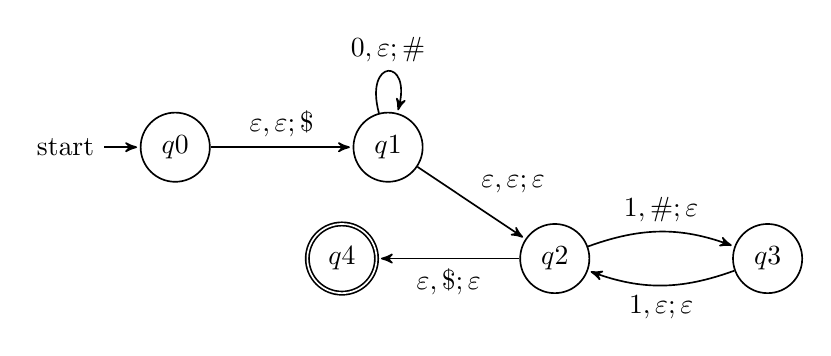
\begin{tikzpicture}[->,>=stealth',shorten >=1pt, auto, node distance=2cm, semithick]
    \tikzstyle{every state}=[text=black, fill=none]
    
    \node[initial,state] (q0)          {$q0$};
    \node[state]         (q1) [right of=q0, xshift=20pt] {$q1$};
    \node[state]         (q2) [below right of=q1, xshift=20pt] {$q2$};
    \node[state]         (q3) [right of=q2, xshift=20pt] {$q3$};
    \node[state,accepting]         (q4) [left of=q2, xshift=-20pt] {$q4$};
    
    \path (q0) edge [bend left=0] node {$\varepsilon, \varepsilon; \$$} (q1)
        (q1) edge  [loop above] node {$0, \varepsilon; \#$} (q1)
        (q1) edge [bend left=0] node {$\varepsilon, \varepsilon; \varepsilon$} (q2)
        (q2) edge  [bend left=20] node [midway, above] {$1, \#; \varepsilon$} (q3)
        (q3) edge  [bend left=20] node [midway, below] {$1, \varepsilon; \varepsilon$} (q2)
        (q2) edge  [bend left=0] node {$\varepsilon, \$; \varepsilon$} (q4)
    ;
\end{tikzpicture}
\\
& \\
& \\
\hline
& $\Gamma = \{ \sun, 1\}$ \hspace{2.3in} \\
& \\
& 
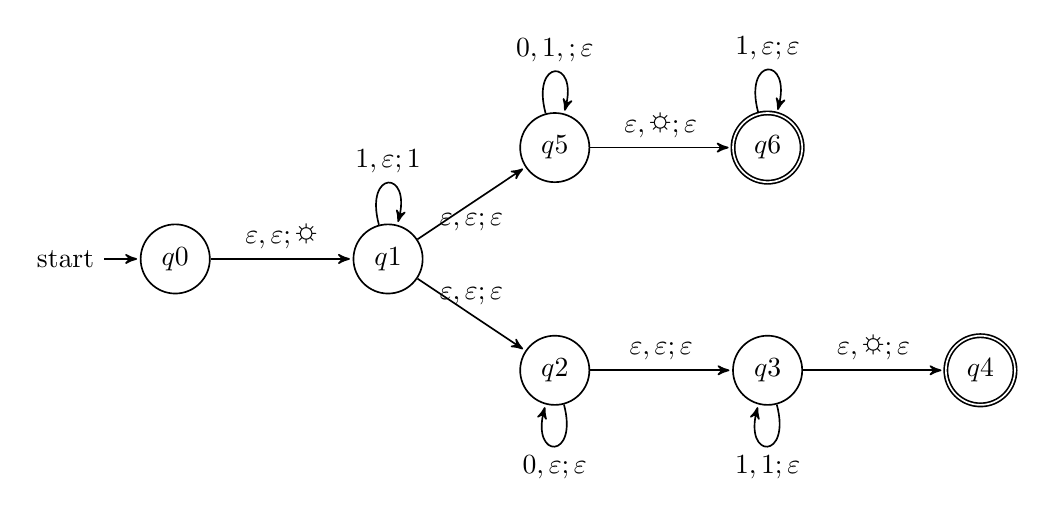
\begin{tikzpicture}[->,>=stealth',shorten >=1pt, auto, node distance=2cm, semithick]
    \tikzstyle{every state}=[text=black, fill=none]
    
    \node[initial,state] (q0)          {$q0$};
    \node[state]         (q1) [right of=q0, xshift=20pt] {$q1$};
    \node[state]         (q2) [below right of=q1, xshift=20pt] {$q2$};
    \node[state]         (q3) [right of=q2, xshift=20pt] {$q3$};
    \node[state,accepting]  (q4) [right of=q3, xshift=20pt] {$q4$};
    \node[state]         (q5) [above right of=q1, xshift=20pt] {$q5$};
    \node[state,accepting]  (q6) [right of=q5, xshift=20pt] {$q6$};
    
    \path (q0) edge [bend left=0] node {$\varepsilon, \varepsilon; \sun$} (q1)
        (q1) edge  [loop above] node {$1, \varepsilon; 1$} (q1)
        (q1) edge [bend left=0] node [below] {$\varepsilon, \varepsilon; \varepsilon$} (q5)
        (q1) edge [bend left=0] node [above]{$\varepsilon, \varepsilon; \varepsilon$} (q2)
        (q5) edge [loop above] node {$0, 1, ; \varepsilon$} (q5)
        (q5) edge [bend left=0] node {$\varepsilon, \sun; \varepsilon$} (q6)
        (q6) edge [loop above] node {$1, \varepsilon; \varepsilon$} (q6)
        (q2) edge [loop below] node {$0, \varepsilon; \varepsilon$} (q2)
        (q2) edge  [bend left=0] node {$\varepsilon, \varepsilon; \varepsilon$} (q3)
        (q3) edge  [loop below] node {$1, 1; \varepsilon$} (q3)
        (q3) edge  [bend left=0] node {$\varepsilon, \sun; \varepsilon$} (q4)
    ;
\end{tikzpicture}
\\
& \\
& \\
\hline
& \\
& \\
& \\
$\{ 0^i 1^j 0^k \mid i,j,k \geq 0 \}$ & \\
& \\
& \\

\end{tabular}
\end{center}
{\it Note: alternate notation is to replace $;$ with $\to$ on arrow labels.}

\newpage
Corollary: for each language $L$ over $\Sigma$, if there is an NFA $N$ with $L(N)=L$
then there is a PDA $M$ with $L(M) = L$

Proof idea: Declare stack alphabet to be $\Gamma = \Sigma$ and then 
don't use stack at all. 


 \vfill

\begin{comment}
{\it Extra practice}: Consider the state diagram of a PDA with input alphabet 
$\Sigma$ and stack alphabet $\Gamma$.

\begin{center}
\begin{tabular}{|c|c|}
\hline
Label & means \\
\hline
$a, b ; c$ when $a \in \Sigma$, $b\in \Gamma$, $c \in \Gamma$ 
& \hspace{3in} \\
& \\
& \\
& \\
& \\
&\\
\hline
$a, \varepsilon ; c$ when $a \in \Sigma$, $c \in \Gamma$ 
& \hspace{3in} \\
& \\
& \\
& \\
& \\
&\\
\hline
$a, b ; \varepsilon$ when $a \in \Sigma$, $b\in \Gamma$
& \hspace{3in} \\
& \\
& \\
& \\
& \\
&\\
\hline
$a, \varepsilon ; \varepsilon$ when $a \in \Sigma$
& \hspace{3in} \\
& \\
& \\
& \\
& \\
&\\
\hline
\end{tabular}
\end{center}


How does the meaning change if $a$ is replaced by $\varepsilon$?
\end{comment}

{\it Big picture}: PDAs are motivated by wanting to add some memory of unbounded size to NFA. How 
do we accomplish a similar enhancement of regular expressions to get a syntactic model that is 
more expressive?

DFA, NFA, PDA: Machines process one input string at a time; the computation of a machine on its input string 
reads the input from left to right.

Regular expressions: Syntactic descriptions of all strings that match a particular pattern; the language 
described by a regular expression is built up recursively according to the expression's syntax

{\bf Context-free grammars}: Rules to produce one string at a time, adding characters from the middle, beginning, 
or end of the final string as the derivation proceeds.\\

\vfill
 \vfill
\section*{Day11}


Regular sets are not the end of the story
\begin{itemize}
    \item Many nice / simple / important sets are not regular
    \item Limitation of the finite-state automaton model: Can't ``count", Can only remember finitely far into the past,
    Can't backtrack, Must make decisions in ``real-time"
    \item We know actual computers are more powerful than this model...
\end{itemize}

The {\bf next} model of computation. Idea: allow some memory of unbounded size. How? 
\begin{itemize}
    \item To generalize regular expressions: {\bf context-free grammars}\\
    \item To generalize NFA: {\bf Pushdown automata}, which is like an NFA with access to a stack: 
    Number of states is fixed, number of entries in stack is unbounded. At each step
    (1) Transition to new state based on current state, letter read, and top letter of stack, then
    (2) (Possibly) push or pop a letter to (or from) top of stack. Accept a string iff
    there is some sequence of states and some sequence of stack contents 
    which helps the PDA processes the entire input string and ends in an accepting state.
\end{itemize}

\vfill

\vfill

Is there a PDA that recognizes the nonregular language $\{0^n1^n \mid n \geq 0 \}$?

\vfill

\newpage

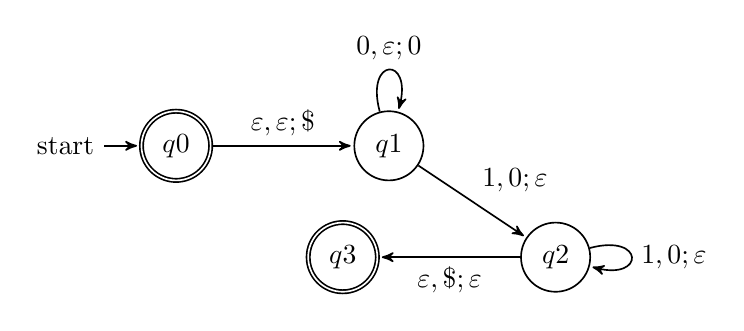
\begin{tikzpicture}[->,>=stealth',shorten >=1pt, auto, node distance=2cm, semithick]
    \tikzstyle{every state}=[text=black, fill=none]
    
    \node[initial,state,accepting] (q0)          {$q0$};
    \node[state]         (q1) [right of=q0, xshift=20pt] {$q1$};
    \node[state]         (q2) [below right of=q1, xshift=20pt] {$q2$};
    \node[state,accepting]         (q3) [left of=q2, xshift=-20pt] {$q3$};
    
    \path (q0) edge [bend left=0] node {$\varepsilon, \varepsilon; \$$} (q1)
        (q1) edge  [loop above] node {$0, \varepsilon; 0$} (q1)
        (q1) edge [bend left=0] node {$1, 0; \varepsilon$} (q2)
        (q2) edge  [loop right] node {$1, 0; \varepsilon$} (q2)
        (q2) edge  [bend left=0] node {$\varepsilon, \$; \varepsilon$} (q3)
    ;
\end{tikzpicture}

The PDA with state diagram above can be informally described as:
\begin{quote}
    Read symbols from the input. As each 0 is read, push it onto the stack. 
    As soon as 1s are seen, pop a 0 off the stack for each 1 read. 
    If the stack becomes empty and we are at the end of the input string, accept the input. 
    If the stack becomes empty and there are 1s left to read, 
    or if 1s are finished while the stack still contains 0s, or if any 0s
    appear in the string following 1s, 
    reject the input.
\end{quote}
    

Trace a computation of this PDA on the input string $01$.

\vfill
    
{\it Extra practice}: Trace the computations of this PDA on the input string $011$.

\vfill

\newpage
A PDA recognizing the set $\{ \hspace{1.5 in} \}$ can be informally described as:
\begin{quote}
    Read symbols from the input. As each 0 is read, push it onto the stack. 
    As soon as 1s are seen, pop a 0 off the stack for each 1 read. 
    If the stack becomes empty and there is exactly one 1 left to read, read that 1 and accept the input. 
    If the stack becomes empty and there are either zero or more than one 1s left to read, 
    or if the 1s are finished while the stack still contains 0s, or if any 0s appear in the input following 1s, 
    reject the input.
\end{quote}
Modify the state diagram below to get a PDA that implements this description:

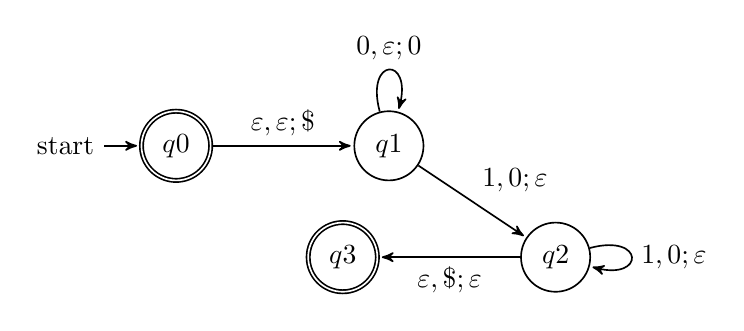
\begin{tikzpicture}[->,>=stealth',shorten >=1pt, auto, node distance=2cm, semithick]
    \tikzstyle{every state}=[text=black, fill=none]
    
    \node[initial,state,accepting] (q0)          {$q0$};
    \node[state]         (q1) [right of=q0, xshift=20pt] {$q1$};
    \node[state]         (q2) [below right of=q1, xshift=20pt] {$q2$};
    \node[state,accepting]         (q3) [left of=q2, xshift=-20pt] {$q3$};
    
    \path (q0) edge [bend left=0] node {$\varepsilon, \varepsilon; \$$} (q1)
        (q1) edge  [loop above] node {$0, \varepsilon; 0$} (q1)
        (q1) edge [bend left=0] node {$1, 0; \varepsilon$} (q2)
        (q2) edge  [loop right] node {$1, 0; \varepsilon$} (q2)
        (q2) edge  [bend left=0] node {$\varepsilon, \$; \varepsilon$} (q3)
    ;
\end{tikzpicture}
    
 \vfill
\section*{Day7}


{\bf Review}: The language recognized by the NFA over $\{a,b\}$ with state diagram


    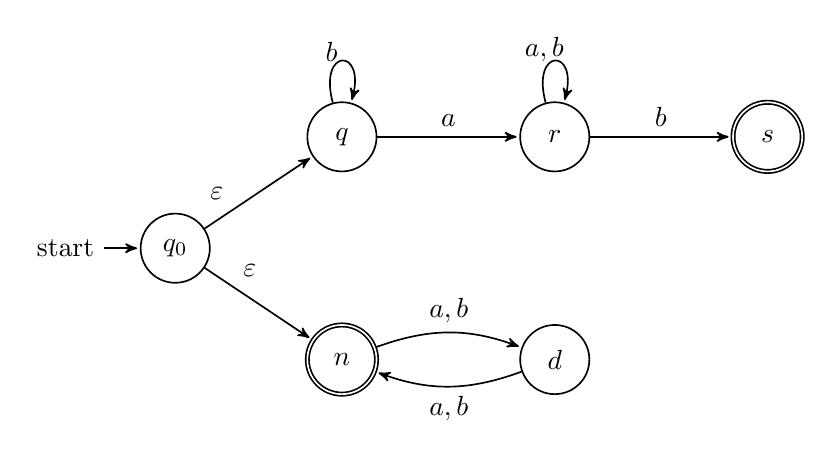
\begin{tikzpicture}[->,>=stealth',shorten >=1pt, auto, node distance=2cm, semithick]
    \tikzstyle{every state}=[text=black, fill=none]
    
    \node[initial,state] (q0)          {$q_0$};
    \node[state]         (q) [above right of=q0, xshift=20pt] {$q$};
    \node[state]         (r) [right of=q, xshift=20pt] {$r$};
    \node[state, accepting]         (s) [right of=r, xshift=20pt] {$s$};
    \node[state, accepting]         (n) [below right of=q0, xshift=20pt] {$n$};
    \node[state]         (d) [right of=n, xshift=20pt] {$d$};
    
    \path (q0) edge  [bend left=0, near start] node {$\varepsilon$} (q)
            edge [bend right=0, near start] node {$\varepsilon$} (n)
        (q) edge [bend left=0] node {$a$} (r)
            edge [loop above, near start] node {$b$} (q)
        (r) edge [bend left=0] node {$b$} (s)
            edge [loop above, near start] node {$a,b$} (r)
        (n) edge [bend left=20] node {$a,b$} (d)
        (d) edge [bend left=20] node {$a,b$} (n)
    ;
    \end{tikzpicture}
is:


\vfill

So far, we know: 
\begin{itemize}
\item The collection of languages that are each recognizable by a 
DFA is {\bf closed} under complementation.

{\it Could we do the same construction with NFA?}

\vspace{100pt}

\item The collection of languages that are each recognizable by a 
NFA is {\bf closed} under union.

{\it Could we do the same construction with DFA?}

\vspace{100pt}

\end{itemize}


\newpage

\vspace{50pt}

Happily, though, an analogous claim is true!

Suppose $A_1, A_2$ are languages over an alphabet $\Sigma$.
{\bf Claim:} if there is a DFA $M_1$ such that $L(M_1) = A_1$ and 
DFA $M_2$ such that $L(M_2) = A_2$, then there is another DFA, let's call it $M$, such that 
$L(M) = A_1 \cup A_2$. {\it Theorem 1.25 in Sipser, page 45}
    
    {\bf Proof idea}:
    
    
    {\bf Formal construction}: 
    
    \vfill

    
    {\bf Example}:  When $A_1 = \{w \mid w~\text{has an $a$ and ends in $b$} \}$ and 
    $A_2 = \{ w \mid w~\text{is of even length} \}$.
    
    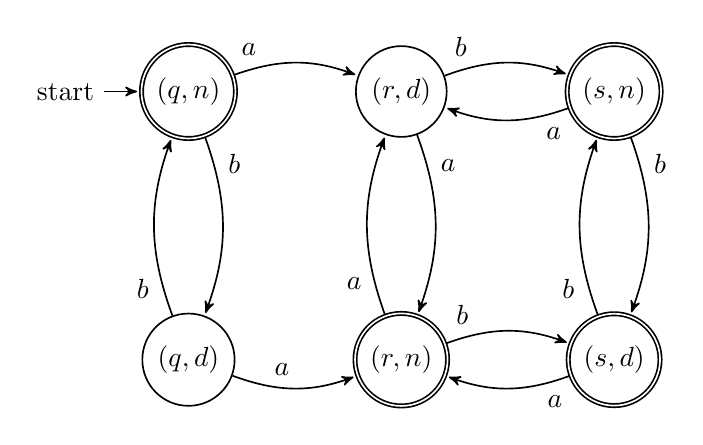
\begin{tikzpicture}[->,>=stealth',shorten >=1pt, auto, node distance=2cm, semithick]
        \tikzstyle{every state}=[text=black, fill=none]
        
        \node[initial,state,accepting] (qn)          {$(q,n)$};
        \node[state]         (qd) [below of=qn, yshift=-40pt] {$(q,d)$};
        \node[state]         (rd) [right of=qn, xshift=20pt] {$(r,d)$};
        \node[state,accepting]         (rn) [right of=qd, xshift=20pt] {$(r,n)$};
        \node[state,accepting]         (sn) [right of=rd, xshift=20pt] {$(s,n)$};
        \node[state,accepting]         (sd) [right of=rn, xshift=20pt] {$(s,d)$};
        
        \path (qn) edge  [bend left=20, near start] node {$b$} (qd)
                edge [bend left=20, near start] node {$a$} (rd)
            (qd) edge [bend left=20, near start] node {$b$} (qn)
                edge [bend right=20, near start] node {$a$} (rn)
            (rn) edge [bend left=20, near start] node {$a$} (rd)
                edge [bend left=20, near start] node {$b$} (sd)
            (rd) edge [bend left=20, near start] node {$a$} (rn)
                edge [bend left=20, near start] node {$b$} (sn)
            (sn) edge [bend left=20, near start] node {$a$} (rd)
                edge [bend left=20, near start] node {$b$} (sd)
            (sd) edge [bend left=20, near start] node {$a$} (rn)
                edge [bend left=20, near start] node {$b$} (sn)
        ;
        \end{tikzpicture}
    
    \newpage
    
    Suppose $A_1, A_2$ are languages over an alphabet $\Sigma$.
    {\bf Claim:} if there is a DFA $M_1$ such that $L(M_1) = A_1$ and 
    DFA $M_2$ such that $L(M_2) = A_2$, then there is another DFA, let's call it $M$, such that 
    $L(M) = A_1 \cap A_2$.  {\it Footnote to Sipser Theorem 1.25, page 46}
    
    {\bf Proof idea}:
    
    
    {\bf Formal construction}: 
    
    \vspace{70pt}


    
 \vfill
\section*{Day8}


So far we have that: 
\begin{itemize}
\item If there is a DFA recognizing a language, there is a DFA recognizing its complement.
\item If there are NFA recognizing two languages, there is a NFA recognizing their union.
\item If there are DFA recognizing two languages, there is a DFA recognizing their union.
\item If there are DFA recognizing two languages, there is a DFA recognizing their intersection.
\end{itemize}

Our goals for today are (1) prove similar results about other set operations, (2) prove that 
NFA and DFA are equally expressive, and therefore (3) define an important class of languages.

\vfill

\newpage
Suppose $A_1, A_2$ are languages over an alphabet $\Sigma$.
{\bf Claim:} if there is a NFA $N_1$ such that $L(N_1) = A_1$ and 
NFA $N_2$ such that $L(N_2) = A_2$, then there is another NFA, let's call it $N$, such that 
$L(N) = A_1 \circ A_2$.

{\bf Proof idea}: Allow computation to move between $N_1$ and $N_2$ ``spontaneously" when reach an accepting state of 
$N_1$, guessing that we've reached the point where the two parts of the string in the set-wise concatenation 
are glued together.


{\bf Formal construction}: Let 
$N_1 = (Q_1, \Sigma, \delta_1, q_1, F_1)$ and $N_2 = (Q_2, \Sigma, \delta_2,q_2, F_2)$
and assume $Q_1 \cap Q_2 = \emptyset$.
Construct $N = (Q, \Sigma, \delta, q_0, F)$ where
\begin{itemize}
    \item $Q = $
    \item $q_0 = $
    \item $F = $
    \item $\delta: Q \times \Sigma_\varepsilon \to \mathcal{P}(Q)$ is defined by, for $q \in Q$ and $a \in \Sigma_{\varepsilon}$:
        \[
            \delta((q,a))=\begin{cases}  
                \delta_1 ((q,a)) &\qquad\text{if } q\in Q_1 \textrm{ and } q \notin F_1\\ 
                \delta_1 ((q,a)) &\qquad\text{if } q\in F_1 \textrm{ and } a \in \Sigma\\ 
                \delta_1 ((q,a)) \cup \{q_2\} &\qquad\text{if } q\in F_1 \textrm{ and } a = \varepsilon\\ 
                \delta_2 ((q,a)) &\qquad\text{if } q\in Q_2
            \end{cases}
        \]
\end{itemize}

\vfill

{\it Proof of correctness would prove that $L(N) = A_1 \circ A_2$ by considering
an arbitrary string accepted by $N$, tracing an accepting computation of $N$ on it, and using 
that trace to prove the string can be written as the result of concatenating two strings, 
the first in $A_1$ and the second in $A_2$; then, taking an arbitrary 
string in $A_1 \circ A_2$ and proving that it is accepted by $N$. Details left for extra practice.}

\vfill
{\bf Application}: A state diagram for a NFA over $\Sigma = \{a,b\}$ 
that recognizes $L ( a^*b)$:


\newpage



Suppose $A$ is a language over an alphabet $\Sigma$.
{\bf Claim:} if there is a NFA $N$ such that $L(N) = A$, then there is another NFA, let's call it $N'$, such that 
$L(N') = A^*$.

{\bf Proof idea}: Add a fresh start state, which is an accept state. Add spontaneous 
moves from each (old) accept state to the old start state.

{\bf Formal construction}: Let 
$N = (Q, \Sigma, \delta, q_1, F)$ and assume $q_0 \notin Q$.
Construct $N' = (Q', \Sigma, \delta', q_0, F')$ where
\begin{itemize}
    \item $Q' = Q \cup \{q_0\}$
    \item $F' = F \cup \{q_0\}$
    \item $\delta': Q' \times \Sigma_\varepsilon \to \mathcal{P}(Q')$ is defined by, for $q \in Q'$ and $a \in \Sigma_{\varepsilon}$:
        \[
            \delta'((q,a))=\begin{cases}  
                \delta ((q,a)) &\qquad\text{if } q\in Q \textrm{ and } q \notin F\\ 
                \delta ((q,a)) &\qquad\text{if } q\in F \textrm{ and } a \in \Sigma\\ 
                \delta ((q,a)) \cup \{q_1\} &\qquad\text{if } q\in F \textrm{ and } a = \varepsilon\\ 
                \{q_1\} &\qquad\text{if } q = q_0 \textrm{ and } a = \varepsilon \\
                \emptyset &\qquad\text{if } q = q_0 \textrm { and } a \in \Sigma
            \end{cases}
        \]
\end{itemize}


{\it Proof of correctness would prove that $L(N') = A^*$ by considering
an arbitrary string accepted by $N'$, tracing an accepting computation of $N'$ on it, and using 
that trace to prove the string can be written as the result of concatenating some number of strings, 
each of which is in $A$; then, taking an arbitrary 
string in $A^*$ and proving that it is accepted by $N'$. Details left for extra practice.}


{\bf Application}: A state diagram for a NFA over $\Sigma = \{a,b\}$ 
that recognizes $L (( a^*b)^* )$:

\vfill
\newpage
Suppose $A$ is a language over an alphabet $\Sigma$.
{\bf Claim:} if there is a NFA $N$ such that $L(N) = A$ then 
there is a DFA $M$ such that $L(M) = A$.

{\bf Proof idea}: States in $M$ are ``macro-states" -- collections of states from $N$ -- 
that represent the set of possible states a computation of $N$ might be in.


{\bf Formal construction}: Let $N = (Q, \Sigma, \delta, q_0, F)$.  Define 
\[
M = (~ \mathcal{P}(Q), \Sigma, \delta', q',  \{ X \subseteq Q \mid X \cap F \neq \emptyset \}~ )
\]
where $q' = \{ q \in Q \mid \text{$q = q_0$ or is accessible from $q_0$ by spontaneous moves in $N$} \}$
and 
\[
    \delta' (~(X, x)~) = \{ q \in Q \mid q \in \delta( ~(r,x)~) ~\text{for some $r \in X$ or is accessible 
from such an $r$ by spontaneous moves in $N$} \}
\]


Consider the state diagram of an NFA over $\{a,b\}$. Use the ``macro-state'' construction 
to find an equivalent DFA.

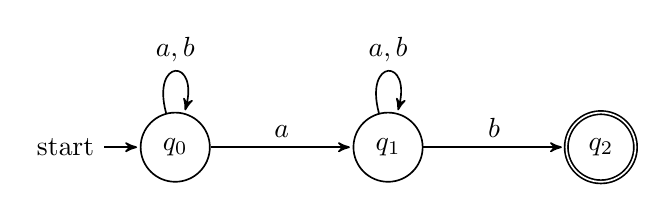
\begin{tikzpicture}[->,>=stealth',shorten >=1pt, auto, node distance=2cm, semithick]
    \tikzstyle{every state}=[text=black, fill=none]
    
    \node[initial,state] (q0)          {$q_0$};
    \node[state]         (q1) [right of=q0, xshift=20pt] {$q_1$};
    \node[state,accepting]         (q2) [right of=q1, xshift=20pt] {$q_2$};
    
    \path (q0) edge  [loop above] node {$a,b$} (q0)
            edge [bend left=0] node {$a$} (q1)
        (q1) edge [loop above] node {$a,b$} (q1)
            edge [bend left=0] node {$b$} (q2)
    ;
    \end{tikzpicture}

\vfill

Consider the state diagram of an NFA over $\{0,1\}$. Use the ``macro-state'' construction 
to find an equivalent DFA.

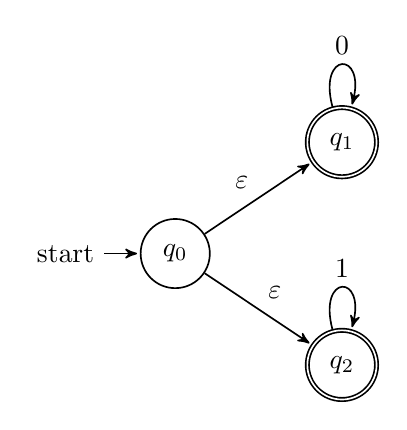
\begin{tikzpicture}[->,>=stealth',shorten >=1pt, auto, node distance=2cm, semithick]
    \tikzstyle{every state}=[text=black, fill=none]
    
    \node[initial,state] (q0)          {$q_0$};
    \node[state,accepting]         (q1) [above right of=q0, xshift=20pt] {$q_1$};
    \node[state,accepting]         (q2) [below right of=q0, xshift=20pt] {$q_2$};
    
    \path (q0)  edge [bend left=0] node {$\varepsilon$} (q1)
        (q0) edge [bend left = 0] node {$\varepsilon$} (q2)
        (q1) edge [loop above] node {$0$} (q1)
        (q2) edge [loop above] node {$1$} (q2)
    ;
    \end{tikzpicture}

\vfill

Note: We can often prune the DFAs that result from the ``macro-state'' constructions to get an 
equivalent DFA with fewer states (e.g.\ only the ``macro-states" reachable from the start state).

\newpage


{\bf The class of regular languages}

Fix an alphabet $\Sigma$. For each language $L$ over $\Sigma$:
\begin{center}
\begin{tabular}{cc}
    {\bf There is a DFA over $\Sigma$ that recognizes $L$}&$\exists M ~(M \textrm{ is a DFA and } L(M) = A)$\\
    {\it if and only if}&\\
    {\bf There is a NFA over $\Sigma$ that recognizes $L$}&$\exists N ~(N \textrm{ is a NFA and } L(N) = A)$\\
    {\it if and only if}&\\
    {\bf There is a regular expression over $\Sigma$ that describes $L$} &$\exists R ~(R \textrm{ is a regular expression and } L(R) = A)$\\
\end{tabular}
\end{center}

A language is called {\bf regular} when any (hence all) of the above three conditions are met.

We already proved that DFAs and NFAs are equally expressive. It remains to prove that regular expressions 
are too.

Part 1: Suppose $A$ is a language over an alphabet $\Sigma$.
If there is a regular expression $R$ such that $L(R) = A$, then there is a NFA, let's call it $N$, such that 
$L(N) = A$.

{\bf Structural induction}: Regular expression is built from basis regular expressions using inductive steps
(union, concatenation, Kleene star symbols). Use constructions to mirror these in NFAs.


{\bf Application}: A state diagram for a NFA over $\{a,b\}$ that recognizes $L(a^* (ab)^*)$:

\vfill

Part 2: Suppose $A$ is a language over an alphabet $\Sigma$.
If there is a DFA $M$ such that $L(M) = A$, then there is a regular expression, let's call it $R$, such that 
$L(R) = A$.

{\bf Proof idea}: Trace all possible paths from start state to accept state.  Express labels of these paths
as regular expressions, and union them all.

\begin{enumerate}
\item Add new start state with $\varepsilon$ arrow to old start state.
\item Add new accept state with $\varepsilon$ arrow from old accept states.  Make old accept states
non-accept.
\item Remove one (of the old) states at a time: modify regular expressions on arrows that went through removed
state to restore language recognized by machine.
\end{enumerate}

{\bf Application}: Find a regular expression describing the language recognized by the DFA with 
state diagram

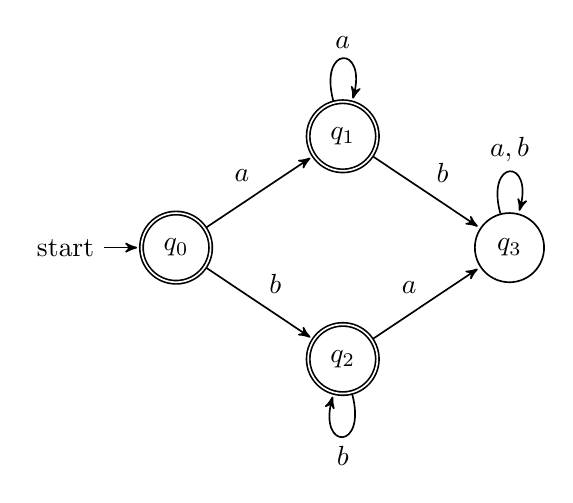
\begin{tikzpicture}[->,>=stealth',shorten >=1pt, auto, node distance=2cm, semithick]
    \tikzstyle{every state}=[text=black, fill=none]
    
    \node[initial,state,accepting] (q0)          {$q_0$};
    \node[state,accepting]         (q1) [above right of=q0, xshift=20pt] {$q_1$};
    \node[state,accepting]         (q2) [below right of=q0, xshift=20pt] {$q_2$};
    \node[state]                   (q3) [below right of=q1, xshift=20pt] {$q_3$};
    
    \path (q0)  edge [bend left=0] node {$a$} (q1)
        (q0) edge [bend left = 0] node {$b$} (q2)
        (q1) edge [loop above] node {$a$} (q1)
        (q1) edge [bend left=0] node {$b$} (q3)
        (q2) edge [loop below] node {$b$} (q2)
        (q2) edge [bend left=0] node {$a$} (q3)
        (q3) edge [loop above] node {$a,b$} (q3)
    ;
    \end{tikzpicture}

\vfill \vfill
\end{document}